\def\linkdethi{} %Đường link cần dẫn tới
\anmaQR
%%%%%%%%%%%%%%%%%%%%%%%%
\def\toanlop{12}
\def\thoigian{90}
\def\namhoc{2025 - 2026}
\begin{dethi}
	{Bộ GD\&ĐT}
	{VTED ft KING EDU}
	{TDMT15}
	{Đề thi thử THPTQG 2026}
\end{dethi}
\caulc
\Opensolutionfile{ans}[ans/ansTN-Dung]
%%%=============EX_1=============%%%
\begin{ex}%[2H2H1-2]%[TDMT15]%[Mui Doan]
	\immini[thm]{Cho hình lăng trụ $ABC.A'B'C'$. Phát biểu nào sau đây là đúng?
		\choice
		{$\overrightarrow{B'A'}+\overrightarrow{AC}=\overrightarrow{B'C}$}
		{\True $\overrightarrow{BA}+\overrightarrow{A'C'}=\overrightarrow{BC}$}
		{$\overrightarrow{BA}+\overrightarrow{AC'}=\overrightarrow{B'C}$}
		{$\overrightarrow{BA}+\overrightarrow{A'B'}=\overrightarrow{BB'}$}}{
		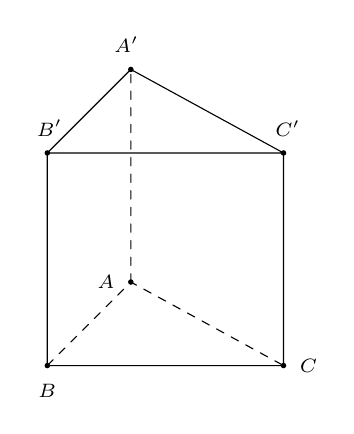
\begin{tikzpicture}[scale=1,line join=round,line cap=round,declare function={a=3; b=0.5*a; h=0.9*a;}]
			\path (0:0) coordinate (A)
			(-135:b) coordinate (B)
			++(a,0) coordinate (C)
			\foreach \x in {A,B,C}{(\x)++(90:h) coordinate (\x1)};
			\draw[dashed] (B)--(A)--(C)
			(A)--(A1);
			\draw (B1)--(A1)--(C1)--cycle
			(B)--(B1)
			(C1)--(C)--(B);
			\foreach \x/\goc/\t in {A/180/A,B/-90/B,C/0/C,A1/100/A',B1/85/B',C1/80/C'}
			\fill (\x) circle (1pt) node[shift={(\goc:9pt)},font=\scriptsize]{$\t$};
		\end{tikzpicture}
	}
	\loigiai{
		Xét từng mệnh đề
		\begin{itemize}
			\item Vì $ACC'A'$ là hình bình hành nên $\overrightarrow{AC} = \overrightarrow{A'C'}$. \\ Do đó $\overrightarrow{B'A'} + \overrightarrow{AC} = \overrightarrow{B'A'} + \overrightarrow{A'C'} = \overrightarrow{B'C'}$.
			\item Theo tính chất lăng trụ ta có $\overrightarrow{A'C'} = \overrightarrow{AC}$. \\ Do đó theo quy tắc ba điểm, ta có $\overrightarrow{BA} + \overrightarrow{A'C'} = \overrightarrow{BA} + \overrightarrow{AC} = \overrightarrow{BC}$.
			\item Theo quy tắc ba điểm, ta có $\overrightarrow{BA} + \overrightarrow{AC'} = \overrightarrow{BC'}$.
			\item Vì $ABB'A'$ là hình bình hành nên $\overrightarrow{A'B'} = \overrightarrow{AB}$. \\ Do đó $\overrightarrow{BA} + \overrightarrow{A'B'} = \overrightarrow{BA} + \overrightarrow{AB} = \overrightarrow{BB} = \overrightarrow{0}$.
		\end{itemize}
	}
\end{ex}
%%%=============================%%%

%%%=============EX_2=============%%%
\begin{ex}%[2H2H2-2]%[TDMT15]%[Huỳnh Trí Thiện]
	\immini[thm]{Cho hình hộp $ABCD.A'B'C'D'$. Đường thẳng $AB$ không song song với mặt phẳng nào sau đây?
		\choice
		{$\left(A'B'C'D'\right)$}
		{$\left(CC'D'D\right)$}
		{\True $\left(B'D'C\right)$}
		{$\left(A'B'CD\right)$}}{
		\begin{tikzpicture}[declare function={a=3; b=0.45*a; h=0.65*a;}]
			\path (0:0) coordinate (A)
			(220:b) coordinate (B)
			($(B)+(a,0)$) coordinate (C)
			(a,0) coordinate (D)
			\foreach \x in {A,B,C,D}{(\x)++(70:h) coordinate (\x1)};
			\draw[dashed] (A1)--(A)--(B)
			(A)--(D);
			\draw (B1)--(A1)--(D1)--(C1)
			(D1)--(D)--(C)
			(B)--(C)--(C1)--(B1)--cycle;
			\foreach \x/\goc/\t in {A/-90/A,B/-90/B,C/-90/C,D/0/D,A1/90/A',B1/90/B',C1/90/C',D1/90/D'}
			\fill (\x) circle (1pt) node[shift={(\goc:7pt)},font=\scriptsize]{$\t$};
		\end{tikzpicture}
	}
	\loigiai{
		Xét từng mệnh đề
		\begin{itemize}
			\item Ta có $AB \parallel A'B'$ (tính chất hình hộp) và $A'B' \subset \left(A'B'C'D'\right)$. Suy ra $AB \parallel \left(A'B'C'D'\right)$.
			\item Ta có $AB \parallel CD$ (tính chất hình hộp) và $CD \subset \left(CC'D'D\right)$. Suy ra $AB \parallel \left(CC'D'D\right)$.
			\item Giả sử $AB \parallel \left(B'D'C\right)$.\\ Vì $AB \parallel CD$ nên $CD \parallel \left(B'D'C\right)$ hoặc $CD \subset \left(B'D'C\right)$.\\ Mặt khác, $C \in \left(B'D'C\right)$ nên bắt buộc $CD \subset \left(B'D'C\right)$.\\ Suy ra $D \in \left(B'D'C\right)$ (tức là $4$ điểm $B'$, $D'$, $C$, $D$ đồng phẳng).\\ Điều này vô lý vì hai đường thẳng $B'D'$ và $CD$ chéo nhau.\\ Do đó đường thẳng $AB$ không song song với mặt phẳng $\left(B'D'C\right)$.
			\item Ta có $AB \parallel CD$ và $CD \subset \left(A'B'CD\right)$. Suy ra $AB \parallel \left(A'B'CD\right)$.
		\end{itemize}
		Vậy đường thẳng $AB$ không song song với mặt phẳng $\left(B'D'C\right)$.
	}
\end{ex}
%%%=============================%%%

%%%=============EX_3=============%%%
\begin{ex}%[2D4H1-2]%[TDMT15]%[Chu Hà]
	Họ nguyên hàm của hàm số $f(x)=x^3$ là
	\choice
	{$\dfrac{1}{4}x^3 + C$}
	{$x^4 + C$}
	{$\dfrac{1}{3}x^4 + C$}
	{\True $\dfrac{1}{4}x^4 + C$}
	\loigiai{
		Họ nguyên hàm của hàm số $f(x)=x^3$ là $\displaystyle\int f(x) \mathrm{\,d}x = \displaystyle\int x^3 \mathrm{\,d}x = \dfrac{x^4}{4}+C$.
	}
\end{ex}
%%%=============================%%%

%%%=============EX_4=============%%%
\begin{ex}%[1D5N1-3]%[TDMT15]%[Nguyễn Tấn Linh]
	Cho hai mẫu số liệu ghép nhóm $M_1$, $M_2$ với bảng tần số ghép nhóm như sau:
	\begin{center}
		\begin{tabular}{|c|c|c|c|c|c|c|c|}
			\hline
			\multirow{2}{*}{$M_1$} & Nhóm & $[3;4)$ & $[4;5)$ & $[5;6)$ & $[6;7)$ & $[7;8)$ & $[8;9)$ \\
			\cline{2-8}
			& Tần số & $3$ & $5$ & $4$ & $6$ & $1$ & $4$ \\
			\hline
			\multirow{2}{*}{$M_2$} & Nhóm & $[2;3)$ & $[3;4)$ & $[4;5)$ & $[5;6)$ & $[6;7)$ & $[7;8)$ \\
			\cline{2-8}
			& Tần số & $7$ & $3$ & $5$ & $4$ & $6$ & $1$ \\
			\hline
		\end{tabular}
	\end{center}
	So sánh trung bình cộng $\overline{x}_1$, $\overline{x}_2$ của $M_1$, $M_2$ thì thấy
	\choice
	{\True $\overline{x}_1 > \overline{x}_2$}
	{$\overline{x}_1 = \overline{x}_2$}
	{$\overline{x}_1 < \overline{x}_2$}
	{$\overline{x}_2 = 2\overline{x}_1 - 3$}
	\loigiai{
		Mẫu số liệu $M_1$ có cỡ mẫu $n_1 = 3 + 5 + 4 + 6 + 1 + 4 = 23$.\\
		Số trung bình của mẫu $M_1$ là
		\[\overline{x}_1 = \dfrac{3 \cdot 3{,}5 + 5 \cdot 4{,}5 + 4 \cdot 5{,}5 + 6 \cdot 6{,}5 + 1 \cdot 7{,}5 + 4 \cdot 8{,}5}{23} = \dfrac{135{,}5}{23} \approx 5{,}89.\]
		Mẫu số liệu $M_2$ có cỡ mẫu $n_2 = 7 + 3 + 5 + 4 + 6 + 1 = 26$.\\
		Số trung bình của mẫu $M_2$ là
		\[\overline{x}_2 = \dfrac{7 \cdot 2{,}5 + 3 \cdot 3{,}5 + 5 \cdot 4{,}5 + 4 \cdot 5{,}5 + 6 \cdot 6{,}5 + 1 \cdot 7{,}5}{26} = \dfrac{119}{26} \approx 4{,}58.\]
		Do đó $\overline{x}_1 > \overline{x}_2$.
	}
\end{ex}
%%%=============================%%%

%%%=============EX_5=============%%%
\begin{ex}%[2H5N2-3]%[TDMT15]%[Phạm Hải Dương]
	Trong không gian $Oxyz$, cho đường thẳng $d \colon \dfrac{x-1}{2}=\dfrac{y+1}{-3}=\dfrac{z-2}{1}$. Hỏi vectơ nào sau đây là một vectơ chỉ phương của $d$?
	\choice
	{$\overrightarrow{v}_1 = (2; 3; 1)$}
	{\True $\overrightarrow{v}_2 = (4; -6; 2)$}
	{$\overrightarrow{v}_3 = (2; -3; -1)$}
	{$\overrightarrow{v}_4 = (-2; 3; 1)$}
	\loigiai{
		Vectơ chỉ phương của đường thẳng $d$ có dạng là $\overrightarrow{v}=k(2;-3;1)$, với $k\neq 0$.\\
		Ta thấy $\overrightarrow{v}_2=(4;-6;2)=2(2;-3;1)=2\overrightarrow{v}$.\\
		Vậy $\overrightarrow{v}_2$ là một vectơ chỉ phương của đường thẳng $d$.
	}
\end{ex}
%%%=============================%%%

%%%=============EX_6=============%%%
\begin{ex}%[1D2H2-4]%[TDMT15]%[Nguyễn Sơn Thành]
	Cho cấp số cộng $\left(u_n\right)$ có $u_1 = 3$ và công sai $d = -2$. Giá trị $u_6$ bằng
	\choice
	{\True $-7$}
	{$-9$}
	{$13$}
	{$-10$}
	\loigiai{
		Ta có công thức số hạng tổng quát của cấp số cộng $u_n = u_1 + (n-1)d$.\\
		Thay $n = 6$, $u_1 = 3$, $d = -2$ vào công thức ta được
		\[u_6 = u_1 + 5d = 3 + 5 \cdot (-2) = 3 - 10 = -7.\]
		Vậy $u_6 = -7$.
	}
\end{ex}
%%%=============================%%%

%%%=============EX_7=============%%%
\begin{ex}%[1D6H4-2]%[TDMT15]%[Bồ Văn Hậu]
	Nghiệm của phương trình $\log_5 (2x-1)=3$ là
	\choice
	{$x=124$}
	{$x=125$}
	{\True $x=63$}
	{$x=7$}
	\loigiai{
		Điều kiện xác định $2x-1 > 0 \Leftrightarrow x > \dfrac{1}{2}$.\\
		Phương trình đã cho tương đương với
		\[2x-1=5^3 \Leftrightarrow 2x - 1 = 125 \Leftrightarrow 2x = 126 \Leftrightarrow x=63 \text{ (thỏa mãn điều kiện).}\]
		Vậy nghiệm của phương trình là $x=63$.
	}
\end{ex}
%%%=============================%%%

%%%=============EX_8=============%%%
\begin{ex}%[1D1N5-5]%[TDMT15]%[Lê Phúc]
	Tập nghiệm của phương trình $\cos x=0$ là
	\choice
	{\True $S=\left\lbrace\dfrac{\pi}{2}+k\pi\mid k\in \mathbb{Z}\right\rbrace$}
	{$S=\left\lbrace k2\pi\mid k\in \mathbb{Z}\right\rbrace$}
	{$S=\left\lbrace \dfrac{\pi}{2}+k3\pi\mid k\in \mathbb{Z}\right\rbrace$}
	{$S=\left\lbrace k\pi\mid k\in \mathbb{Z}\right\rbrace$}
	\loigiai{
		Ta có $\cos x=0\Leftrightarrow x=\dfrac{\pi}{2}+k\pi$ ($k\in\mathbb{Z}$).\\
		Vậy tập nghiệm của phương trình đã cho là $S=\left\lbrace\dfrac{\pi}{2}+k\pi\mid k\in \mathbb{Z}\right\rbrace$.
	}
\end{ex}
%%%=============================%%%

%%%=============EX_9=============%%%
\begin{ex}%[2D4H3-1]%[TDMT15]%[Trần Văn Thiện]
	Trong mặt phẳng với hệ toạ độ $Oxy$, diện tích $S$ của hình phẳng giới hạn bởi đồ thị của hàm số $y=3x-4$, trục hoành và hai đường thẳng $x=3$, $x=1$ được xác định bằng công thức
	\choice
	{$S=\pi\displaystyle\int\limits_{1}^{3}\left|3x-4\right|\mathrm{\,d}x$}
	{\True $S=\displaystyle\int\limits_{1}^{3}\left|3x-4\right|\mathrm{\,d}x$}
	{$S=\pi\displaystyle\int\limits_{1}^{3}(3x-4)^2\mathrm{\,d}x$}
	{$S=\left|\displaystyle\int\limits_{1}^{3}\left(3x-4\right)\mathrm{\,d}x\right|$}
	\loigiai{
		Diện tích của hình phẳng giới hạn bởi đồ thị của hàm số $y=3x-4$, trục hoành và hai đường thẳng $x=3$, $x=1$ là $S=\displaystyle\int\limits_{1}^{3}\left|3x-4\right|\mathrm{\,d}x$.
	}
\end{ex}
%%%=============================%%%

%%%=============EX_10=============%%%
\begin{ex}%[2H5N1-3]%[TDMT15]%[Đình Nguyên]
	Trong không gian $Oxyz$, mặt phẳng đi qua điểm $A(2; 1; -3)$ và nhận $\overrightarrow{n} = (3; 2; -2)$ làm một vectơ pháp tuyến có phương trình tổng quát là
	\choice
	{$3(x + 2) + 2(y + 1) - 2(z - 3) = 0$}
	{$2(x - 3) + 1(y - 2) - 3(z + 2) = 0$}
	{$2(x + 3) + 1(y + 2) - 3(z - 2) = 0$}
	{\True $3(x - 2) + 2(y - 1) - 2(z + 3) = 0$}
	\loigiai{
		Mặt phẳng đi qua điểm $A(2; 1; -3)$ và nhận $\overrightarrow{n} = (3; 2; -2)$ làm vectơ pháp tuyến có phương trình là
		\[3(x - 2) + 2(y - 1) - 2(z + 3) = 0.\]
	}
\end{ex}
%%%=============================%%%

%%%=============EX_11=============%%%
\begin{ex}%[1H8H7-2]%[TDMT15]%[Huynh Quốc Đạt]
	Cho hình chóp $S.ABC$ có cạnh $SA$ vuông góc với mặt phẳng $(ABC)$, tam giác $ABC$ vuông tại $A$ và $SA=6$, $AB=3$, $BC=5$. Thể tích của khối chóp $S.ABC$ bằng
	\choice
	{\True $12$}
	{$30$}
	{$15$}
	{$60$}
	\loigiai{
		\immini{Tam giác $ABC$ vuông tại $A$ nên $AC=\sqrt{BC^2-AB^2}=\sqrt{5^2-3^2}=4$.\\
			Thể tích của khối chóp $S.ABC$ là
			\[V_{S.ABC}=\dfrac{1}{3}S_{ABC}\cdot h =\dfrac{1}{3}\cdot \left(\dfrac{1}{2}\cdot AB\cdot AC\right)\cdot SA=\dfrac{1}{3}\cdot \left(\dfrac{1}{2}\cdot 3\cdot 4\right)\cdot 6=12\,\,(\text{đơn vị thể tích}).\]}{
			\begin{tikzpicture}[declare function={a=2; b=0.45*a; h=0.65*a;}]
				\path (0,0) coordinate (A)
				(a,0) coordinate (C)
				(-45:b) coordinate (B)
				($(A)+(0,h)$) coordinate (S);
				\foreach \x/\y/\z in {B/A/S,C/A/S,B/A/C}{
					\path pic[draw,angle radius=3pt]{right angle=\x--\y--\z};
				}
				\draw[dashed] (A)--(C);
				\draw (S)--(B)
				(S)--(A)--(B)--(C)--cycle;
				\foreach \x/\goc in {S/90,A/190,B/-90,C/0}
				\fill (\x) node[shift={(\goc:7pt)},font=\scriptsize]{$\x$} circle (1pt);
			\end{tikzpicture}
		}
	}
\end{ex}
%%%=============================%%%

%%%=============EX_12=============%%%
\begin{ex}%[2D1N4-1]%[TDMT15]%[Nguyễn Trí Minh Tuấn]
	\immini[thm]{Cho hàm số $y=\dfrac{ax+b}{cx+d}$ ($ac\ne 0$, $ad-bc\ne 0$) có đồ thị như hình bên. Đường tiệm cận đứng của đồ thị hàm số đã cho có phương trình là
		\choice
		{$y=2$}
		{\True $x=1$}
		{$y=1$}
		{$x=2$}
	}{
		\begin{tikzpicture}[scale=.5,line cap=butt,line join=miter,>=stealth]
			\draw[->] (-3,0)--(5,0)
			node[shift={(-100:7pt)},font=\normalsize]{$x$};
			\draw[->] (0,-3)--(0,5)
			node[shift={(180:7pt)},font=\normalsize]{$y$};
			\draw (5pt,0) |- (0,5pt)
			(0,0) node[shift={(225:9pt)},font=\normalsize]{$O$};
			\foreach \x in {1}{
				\draw (\x,1.5pt)--(\x,-1.5pt) node[font=\scriptsize,below left,fill=white,inner sep=1pt]{\x};
			}
			\foreach \y in {2}{
				\draw (1.5pt,\y)--(-1.5pt,\y) node[font=\scriptsize,below left,fill=white,inner sep=1pt]{\y};
			}
			\tikzset{declare function={f (\x)=2-1/((\x)-1);}}
			\begin{scope}
				\clip (-3,-3) rectangle (5,5);
				\draw[dashed,red] (1,-3) -- (1,5);
				\draw[dashed,red] (-3,2) -- (5,2);
				\draw[blue,smooth,samples=100,domain=-3:0.85] plot (\x,{f (\x)});
				\draw[blue,smooth,samples=100,domain=1.15:5] plot (\x,{f (\x)});
			\end{scope}
		\end{tikzpicture}
	}
	\loigiai{
		Quan sát đồ thị, ta thấy đường thẳng tiệm cận đứng của đồ thị đi qua điểm có hoành độ $x=1$.\\
		Do đó tiệm cận đứng của đồ thị hàm số có phương trình là $x=1$.
	}
\end{ex}
%%%=============================%%%
\Closesolutionfile{ans}

\cauds
\Opensolutionfile{ans}[ans/ansTN-DungSai]
%%%=============EX_13=============%%%
\begin{ex}%[2D1V5-8]%[TDMT15]%[Dương Công Tạo]
	Nghiên cứu một quần thể vi khuẩn được nuôi cấy trong phòng thí nghiệm. Người ta cung cấp nồng độ dinh dưỡng $D$ (đơn vị: mg/l) thay đổi theo thời gian sau $t$ giờ ($t \ge 0$) được mô hình hóa bởi hàm số $D(t)=\dfrac{13t+2}{t+4}$. Biết rằng tốc độ sinh trưởng $L$ của vi khuẩn phụ thuộc vào nồng độ dinh dưỡng theo hàm số $L(D)= \dfrac{20D}{D+3}$. Khi thời gian $t$ kéo dài, tốc độ sinh trưởng $L$ tăng dần và ổn định ở ngưỡng $L_{\max}$.
	\choiceTF[t]
	{\True Nồng độ dinh dưỡng $D(t)$ tăng dần theo thời gian}
	{\True Tốc độ sinh trưởng ban đầu của quần thể vi khuẩn là $2{,}86$ con/giờ (\textit{làm tròn kết quả đến hàng phần trăm})}
	{Tốc độ sinh trưởng ổn định ứng với $L_{\max} = 18{,}5$ (con/giờ)}
	{\True Gọi $t_0$ là giá trị thời gian để tốc độ sinh trưởng vừa bằng $80\%$ giá trị $L_{\max}$. Khi đó ta có $t_0 = 2{,}73$ (\textit{làm tròn kết quả đến hàng phần trăm})}
	\loigiai{
		\begin{itemchoice}
			\itemch Xét hàm số $D(t)= \dfrac{13t + 2}{t + 4}$ trên nửa khoảng $[0; +\infty)$.\\
			Ta có $D'(t)=\dfrac{50}{(t + 4)^2} > 0$, $\forall t \ge 0$.\\
			Do đó, hàm số $D(t)$ luôn đồng biến (tăng dần) trên $[0; +\infty)$.
			\itemch Tại thời điểm ban đầu $t = 0$, ta có
			\begin{itemize}
				\item Nồng độ dinh dưỡng ban đầu $D(0) = \dfrac{13 \cdot 0 + 2}{0 + 4} = 0{,}5$ (mg/l).
				\item Tốc độ sinh trưởng ban đầu $L(0{,}5) = \dfrac{20 \cdot 0{,}5}{0{,}5 + 3} = \dfrac{10}{3{,}5} = \dfrac{20}{7} \approx 2{,}86$ (con/giờ).
			\end{itemize}
			\itemch Khi thời gian $t$ kéo dài nghĩa là $t \to +\infty$ thì nồng độ dinh dưỡng $D$ tiến dần đến giá trị giới hạn
			\[\lim\limits_{t \to +\infty} D(t)= \lim\limits_{t \to +\infty} \dfrac{13t + 2}{t + 4} = 13 \text{ (mg/l)}.\]
			Khi đó, tốc độ sinh trưởng $L$ sẽ ổn định ở ngưỡng
			\[L_{\max} = \lim\limits_{D \to 13} L(D)= \dfrac{20 \cdot 13}{13 + 3} = \dfrac{260}{16} = 16{,}25 \text{ (con/giờ)}.\]
			\itemch Ta có $L = 80\% \cdot L_{\max} = 0{,}8 \cdot 16{,}25 = 13$.\\
			Mặt khác $L = \dfrac{20D}{D+ 3} \Rightarrow \dfrac{20D}{D+3} = 13 \Leftrightarrow 20D = 13D + 39 \Leftrightarrow 7D = 39 \Leftrightarrow D = \dfrac{39}{7}$.\\
			Với $D = \dfrac{39}{7}$, ta suy ra thời gian $t_0$
			\[\dfrac{13t_0+2}{t_0+4} = \dfrac{39}{7} \Leftrightarrow 91t_0 + 14 = 39t_0 + 156 \Leftrightarrow 52t_0 = 142 \Leftrightarrow t_0 = \dfrac{71}{26} \approx 2{,}73 \text{ (giờ)}.\]
		\end{itemchoice}
	}
\end{ex}
%%%=============================%%%

%%%=============EX_14=============%%%
\begin{ex}%[2D6V2-4]%[TDMT15]%[Hà Văn Hảo]
	Một bài toán giả tưởng và trong bài chỉ xét những người ở độ tuổi $30$. Theo một nguồn thống kê nào đó cho thấy cứ $200$ người có $20$ người thành công rực rỡ, trong đó chỉ có $6$ người là có học lực giỏi chăm chỉ phấn đấu. Chọn ngẫu nhiên một người từ $200$ người được thống kê. Gọi $A$ là biến cố chọn được người thành công rực rỡ, $B$ là biến cố chọn được người có học lực giỏi chăm chỉ phấn đấu. Trong thực tế thì xét cùng ở độ tuổi $30$, số lượng người có học lực giỏi chăm chỉ phấn đấu chỉ bằng $10\%$ số lượng người còn lại.
	\choiceTF[t]
	{\True $\mathrm{P}(A) = 0{,}1$}
	{\True $\mathrm{P}(B \mid A) = 0{,}3$}
	{$\mathrm{P}(B) = \dfrac{1}{10}$}
	{\True Tỉ lệ người giỏi chăm chỉ phấn đấu sẽ thành công rực rỡ gấp $4{,}3$ lần tỉ lệ người còn lại sẽ thành công rực rỡ (\textit{làm tròn kết quả đến hàng phần mười})}
	\loigiai{
		Gọi không gian mẫu $\Omega$ là tập hợp $200$ người được thống kê.\\ Ta có $n(\Omega) = 200$.\\
		Xét các biến cố như đề bài đã gọi
		\begin{itemize}
			\item $A$: \lq\lq Người được chọn thành công rực rỡ\rq\rq. Theo giả thiết $n(A) = 20$.
			\item $B$: \lq\lq Người được chọn có học lực giỏi, chăm chỉ phấn đấu\rq\rq.
			\item $A \cap B$: \lq\lq Người được chọn vừa thành công rực rỡ, vừa có học lực giỏi, chăm chỉ phấn đấu\rq\rq. Theo giả thiết $n(A \cap B) = 6$.
		\end{itemize}
		\begin{center}
			\begin{tikzpicture}[
				line join = round,line cap = round,>=stealth,scale=1,inner sep = 1 mm,node distance = 2 cm and 2 cm,
				hcnxanh/.style={rectangle,draw = blue!80,fill = blue!30,minimum width=0.8 cm,minimum height=0.6 cm},
				hcnvang/.style={rectangle,draw = yellow!80,fill = yellow!50,minimum width=0.8 cm,minimum height=0.6 cm},
				hcnnau/.style={rectangle,draw = brown!80,fill = brown!50,minimum width=0.6 cm,minimum height=0.6 cm}]
				\node at (0,0)
				(nodeO) [hcnnau]{$\Omega$};
				\node at (3,2)
				(nodeB) [hcnxanh] {$B$};
				\node at (3,-2)
				(nodeBd) [hcnxanh] {$\overline{B}$};
				\node at (7,3)
				(nodeA1) [hcnvang] {$A$};
				\node at (7,1)
				(nodeAd1) [hcnvang] {$\overline{A}$};
				\node at (7,-1)
				(nodeA2) [hcnvang] {$A$};
				\node at (7,-3)
				(nodeAd2) [hcnvang] {$\overline{A}$};
				\draw[->] (nodeO) to node[above left]{$\dfrac{1}{11}$}
				(nodeB);
				\draw[->] (nodeO) to node[below left]{$\dfrac{10}{11}$}
				(nodeBd);
				\draw[->] (nodeB) to node[above left]{$0{,}33$}
				(nodeA1);
				\draw[->] (nodeB) to node[below left]{$0{,}67$}
				(nodeAd1);
				\draw[->] (nodeBd) to node[above left]{$0{,}077$}
				(nodeA2);
				\draw[->] (nodeBd) to node[below left]{$0{,}923$}
				(nodeAd2);
				\draw[<-,dashed,red] (nodeA1)--(9.5,3)--(9.5,1) node[right]{$\Rightarrow\mathrm{P}
					(A) = 0{,}1$}--(9.5,-1);
				\draw[<-,dashed,red] (nodeA2)--(9.5,-1);
			\end{tikzpicture}
		\end{center}
		\begin{itemchoice}
			\itemch Xác suất chọn được người thành công rực rỡ là
			\begin{align*}
				\mathrm{P}(A) = \dfrac{n(A)}{n(\Omega)} = \dfrac{20}{200} = 0{,}1.
			\end{align*}
			\itemch Theo công thức xác suất có điều kiện, xác suất chọn được người giỏi chăm chỉ phấn đấu biết người đó thành công rực rỡ là
			\begin{align*}
				\mathrm{P}(B \mid A) = \dfrac{n(A \cap B)}{n(A)} = \dfrac{6}{20} = 0{,}3.
			\end{align*}
			\itemch Theo giả thiết thực tế, số lượng người giỏi chăm chỉ phấn đấu ($B$) bằng $10\%$ số lượng người còn lại ($\overline{B}$).\\ Gọi $x$ là số người giỏi chăm chỉ phấn đấu, ta có phương trình
			\begin{align*}
				x = 10\% \cdot (200 - x) \Leftrightarrow x = 0{,}1(200 - x) \Leftrightarrow 1{,}1 x = 20 \Leftrightarrow x = \dfrac{200}{11}.
			\end{align*}
			Xác suất chọn được người giỏi chăm chỉ phấn đấu là
			\begin{align*}
				\mathrm{P}(B) = \dfrac{x}{n(\Omega)} = \dfrac{200/11}{200} = \dfrac{1}{11}.
			\end{align*}
			\itemch Ta cần so sánh hai xác suất có điều kiện $\mathrm{P}(A \mid B)$ và $\mathrm{P}\left(A \mid \overline{B}\right)$.\\
			Tỉ lệ người giỏi chăm chỉ phấn đấu thành công rực rỡ là
			\begin{align*}
				\mathrm{P}(A \mid B) = \dfrac{n(A \cap B)}{n(B)} = \dfrac{6}{\dfrac{200}{11}} = \dfrac{66}{200} = 0{,}33.
			\end{align*}
			Số người không giỏi, không chăm chỉ phấn đấu là $n\left(\overline{B}\right) = 200 - \dfrac{200}{11} = \dfrac{2\,000}{11}$.\\
			Số người thành công rực rỡ nhưng không giỏi chăm chỉ là
			\begin{align*}
				n\left(A \cap \overline{B}\right) = n(A) - n(A \cap B) = 20 - 6 = 14.
			\end{align*}
			Tỉ lệ người không giỏi chăm chỉ phấn đấu nhưng vẫn thành công rực rỡ là
			\begin{align*}
				\mathrm{P}\left(A \mid \overline{B}\right) = \dfrac{n\left(A \cap \overline{B}\right)}{n\left(\overline{B}\right)} = \dfrac{14}{\dfrac{2\,000}{11}} = \dfrac{154}{2\,000} = 0{,}077.
			\end{align*}
			Ta có
			\begin{align*}
				\dfrac{\mathrm{P}(A \mid B)}{\mathrm{P}\left(A \mid \overline{B}\right)} = \dfrac{0{,}33}{0{,}077} = \dfrac{330}{77} = \dfrac{30}{7} \approx 4{,}3.
			\end{align*}
		\end{itemchoice}
	}
\end{ex}
%%%=============================%%%

%%%=============EX_15=============%%%
\begin{ex}%[2D4V3-3]%[TDMT15]%[Văn Minh Thoại]
	Trong mặt phẳng toạ độ $Oxy$, cho hình phẳng $(H)$ giới hạn bởi đường cong $(\omega)$ có phương trình $x^4+y^2-4x^2=0$.
	\choiceTF[t]
	{Đường cong $(\omega)$ có đúng hai điểm chung với trục hoành $Ox$}
	{\True Mọi điểm $M(x ; y)$ nằm trên $(\omega)$ đều thoả mãn $-2\leq x\leq 2$}
	{Diện tích của $(H)$ bằng $11{,}3$ \textit{(làm tròn kết quả đến hàng phần mười)}}
	{\True Thể tích khối tròn xoay thu được khi cho $(H)$ quay quanh trục hoành $Ox$ là $27$ \textit{(làm tròn kết quả đến hàng đơn vị)}}
	\loigiai{
		Từ phương trình đường cong $(\omega)$ ta có $x^4+y^2-4x^2=0 \Leftrightarrow y^2=4x^2-x^4$.
		\begin{itemchoice}
			\itemch
			\immini{Phương trình hoành độ giao điểm của $(\omega)$ và trục hoành $Ox$ ($y=0$) là
				\allowdisplaybreaks
				\begin{align*}
					&x^4 - 4x^2 = 0 \\
					\Leftrightarrow\ & x^2(x^2 - 4) = 0\\
					\Leftrightarrow\ &\hoac{&x = 0 \\ &x = 2 \\ &x = -2.}
				\end{align*}
				Vậy đường cong $(\omega)$ cắt trục hoành tại $3$ điểm phân biệt $(0;0)$, $(2;0)$ và $(-2;0)$.
			}{
				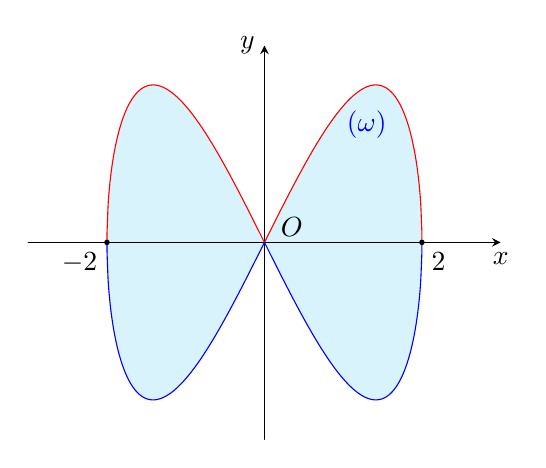
\begin{tikzpicture}[>=stealth,scale=1,line join=round,line cap=round,declare function={f (\x)=abs (\x)*sqrt (4-\x*\x);}]
					\fill[cyan!15]
					(-2,0) -- plot[domain=-1.999:0,samples=150,smooth] (\x,{f (\x)})
					-- plot[domain=0:1.999,samples=150,smooth] (\x,{f (\x)})
					-- (2,0)
					-- plot[domain=1.999:0,samples=150,smooth] (\x,{-f (\x)})
					-- plot[domain=0:-1.999,samples=150,smooth] (\x,{-f (\x)})
					-- cycle;
					\draw[->] (-3,0) -- (3,0) node[below] {$x$};
					\draw[->] (0,-2.5) -- (0,2.5) node[left] {$y$};
					\node at (0,0) [shift=(30:0.4)] {$O$};
					\draw[red]
					(-2,0) -- plot[domain=-1.999:0,samples=150,smooth] (\x,{f (\x)})
					-- plot[domain=0:1.999,samples=150,smooth] (\x,{f (\x)}) -- (2,0);
					\draw[blue]
					(-2,0) -- plot[domain=-1.999:0,samples=150,smooth] (\x,{-f (\x)})
					-- plot[domain=0:1.999,samples=150,smooth] (\x,{-f (\x)}) -- (2,0);
					\fill (2,0) circle (1pt) node[below right] {$2$};
					\fill (-2,0) circle (1pt) node[below left] {$-2$};
					\node[blue] at (1.3,1.5) {$(\omega)$};
				\end{tikzpicture}
			}
			\itemch Vì $y^2\ge 0$ với mọi $y$, nên để tồn tại điểm $M(x;y)$ nằm trên $(\omega)$ thì hoành độ $x$ phải thoả mãn điều kiện
			\allowdisplaybreaks
			\begin{align*}
				4x^2 - x^4 \ge 0 \Leftrightarrow x^2\left(4 - x^2\right) \ge 0 \Leftrightarrow -2 \le x \le 2.
			\end{align*}
			Do đó mọi điểm nằm trên $(\omega)$ đều có hoành độ thỏa mãn $-2\le x\le 2$.
			\itemch Đường cong $(\omega)$ bao gồm hai nhánh đối xứng qua trục hoành là $y = |x|\sqrt{4-x^2}$ và $y = -|x|\sqrt{4-x^2}$ với $x\in[-2;2]$.\\
			Do tính đối xứng qua hai trục tọa độ, diện tích của hình phẳng $(H)$ bằng $4$ lần phần diện tích nằm trong góc phần tư thứ nhất. Khi đó ta có
			\[S = 4\displaystyle\int\limits_{0}^{2} x\sqrt{4-x^2} \mathrm{\,d}x = 4 \left[-\dfrac{1}{3}\sqrt{\left(4-x^2\right)^3} \right] \Bigg|_0^2 = 4 \left[0 - \left(-\dfrac{8}{3}\right) \right] = \dfrac{32}{3} \approx 10{,}7. \]
			\itemch Thể tích khối tròn xoay thu được khi quay $(H)$ quanh trục hoành $Ox$ là
			\allowdisplaybreaks
			\begin{align*}
				V &= \pi \displaystyle\int\limits_{-2}^{2} y^2 \mathrm{\,d}x = \pi \displaystyle\int\limits_{-2}^{2}\left(4x^2 - x^4\right) \mathrm{\,d}x \\
				&= \pi \left(\dfrac{4}{3}x^3 - \dfrac{1}{5}x^5 \right) \Bigg|_{-2}^{2} = \pi \left[\left(\dfrac{32}{3} - \dfrac{32}{5} \right) - \left(-\dfrac{32}{3} + \dfrac{32}{5} \right) \right] \\
				&= \pi \left(\dfrac{64}{15} + \dfrac{64}{15} \right) = \dfrac{128\pi}{15} \approx 27.
			\end{align*}
		\end{itemchoice}
	}
\end{ex}
%%%=============================%%%

%%%=============EX_16=============%%%
\begin{ex}%[2H5V2-8]%[TDMT15]%[Vũ Hồng Toàn]
	\immini[thm]{Trong không gian $Oxyz$, cho một miếng bìa hình vuông $(V)$, chắn không cho ánh sáng đi qua, có cạnh bằng $\sqrt{2}$, có tâm là gốc tọa độ $O$, có bốn đỉnh nằm trên hai trục tọa độ $Ox$, $Oy$. Một vật coi như một hạt nằm tại điểm $A(-6;-3;5)$, mắt người quan sát đặt tại điểm $M(4;2;-3)$.
	}{
		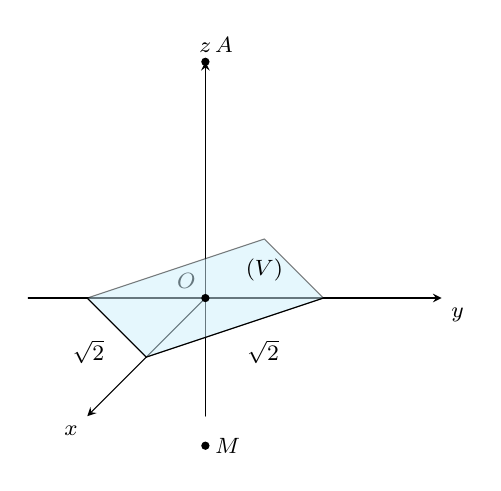
\begin{tikzpicture}[x={(-0.5cm,-0.5cm)},y={(1cm,0cm)},z={(0cm,1cm)},scale=1.5,font=\footnotesize,line join=round,line cap=round,>=stealth]
			\draw[->] (0,0,0) -- (2,0,0) node[below left] {$x$};
			\draw[->] (0,-1.5,0) -- (0,2,0) node[below right] {$y$};
			\draw[->] (0,0,-1) -- (0,0,2) node[above] {$z$};
			\node[above left] at (0,0,0) {$O$};
			\coordinate (E) at (1,0,0);
			\coordinate (F) at (0,1,0);
			\coordinate (G) at (-1,0,0);
			\coordinate (H) at (0,-1,0);
			\draw[fill=cyan!20,opacity=0.5] (E) -- (F) -- (G) -- (H) -- cycle;
			\draw (E) -- (F) node[midway,below right=1pt] {$\sqrt{2}$};
			\draw (E) -- (H) node[midway,below left=1pt] {$\sqrt{2}$};
			\node[below=8pt] at (0,0.5,0.6) {$(V)$};
			\coordinate (A) at (-1.5,-0.75,1.25);
			\coordinate (M) at (1,0.5,-0.75);
			\fill (A) circle (1pt) node[above right] {$A$};
			\fill (M) circle (1pt) node[right] {$M$};
			\fill (0,0,0) circle (1pt);
		\end{tikzpicture}
	}
	\choiceTF[t]
	{\True Một đỉnh của hình vuông có tọa độ là $(1;0;0)$}
	{\True Phương trình tham số của đường thẳng $AM$ là $\heva{&x = -6 + 10t \\& y = -3 + 5t \\& z = 5 - 8t}$}
	{\True Nếu đường thẳng $AM$ cắt mặt phẳng $(Oxy)$ tại điểm $N(a;b;c)$ thì $4a+8b+12c=2$}
	{Người quan sát vẫn nhìn được điểm $A$ mà không bị hình vuông $(V)$ chắn mất tầm nhìn}
	\loigiai{
		\begin{itemchoice}
			\itemch
			\immini{
				Gọi $E$, $F$, $G$, $H$ là bốn đỉnh của hình vuông $(V)$.\\
				Vì các đỉnh nằm trên hai trục tọa độ $Ox$, $Oy$ và hình vuông có tâm là gốc $O(0;0;0)$, nên tọa độ các đỉnh phải có dạng: $E(a;0;0)$, $G(-a;0;0)$, $F(0;a;0)$, $H(0;-a;0)$ với $a > 0$.\\
				Độ dài một cạnh của hình vuông $(V)$ là
				\[EF = \sqrt{a^2 + a^2 + 0} = a\sqrt{2}. \]
				Theo giả thiết, cạnh hình vuông bằng $\sqrt{2}$ nên
				\[a\sqrt{2} = \sqrt{2} \Leftrightarrow a=1. \]
			}{
				\begin{tikzpicture}[x={(-0.5cm,-0.5cm)},y={(1cm,0cm)},z={(0cm,1cm)},scale=1.5,font=\footnotesize,line join=round,line cap=round,>=stealth]
					\draw[->] (0,0,0) -- (2.2,0,0) node[below left] {$x$};
					\draw[->] (0,-1.5,0) -- (0,2.2,0) node[below right] {$y$};
					\draw[->] (0,0,-1.2) -- (0,0,2.2) node[above] {$z$};
					\node[above right] at (0,0,0) {$O$};
					\coordinate (E) at (1,0,0);
					\coordinate (F) at (0,1,0);
					\coordinate (G) at (-1,0,0);
					\coordinate (H) at (0,-1,0);
					\draw[fill=cyan!20,opacity=0.8] (E) -- (F) -- (G) -- (H) -- cycle;
					\draw (E) -- (F) -- (G) -- (H) -- cycle;
					\node[below=2pt] at (E) {$E$};
					\node[above left=2pt] at (E) {$1$};
					\node[below right=2pt] at (F) {$F$};
					\node[above right=2pt] at (F) {$1$};
					\node[above=2pt] at (G) {$G$};
					\node[above left=2pt] at (G) {$-1$};
					\node[above left=2pt] at (H) {$H$};
					\node[below left=2pt] at (H) {$-1$};
					\node at (-0.2,0.4,0) {$(V)$};
					\coordinate (A) at (-1.5,-0.75,1.25);
					\coordinate (M) at (1,0.5,-0.75);
					\coordinate (N) at (0.0625,0.03125,0);
					\draw (A) -- (N);
					\draw[dashed] (N) -- ($(N)!0.4!(M)$);
					\draw ($(N)!0.4!(M)$) -- (M);
					\fill (A) circle (1pt) node[above right] {$A$};
					\fill (M) circle (1pt) node[right] {$M$};
					\fill (N) circle (1pt) node[below right=1pt] {$N$};
					\fill (0,0,0) circle (1pt);
				\end{tikzpicture}
			}
			\noindent Suy ra tọa độ các đỉnh của hình vuông là $(1;0;0)$, $(-1;0;0)$, $(0;1;0)$, $(0;-1;0)$.
			\itemch Đường thẳng $AM$ đi qua hai điểm $A(-6;-3;5)$ và $M(4;2;-3)$.\\
			Vectơ chỉ phương của đường thẳng $AM$ là
			\[\overrightarrow{AM} = (x_M - x_A; y_M - y_A; z_M - z_A) = (10; 5; -8). \]
			Suy ra phương trình tham số của đường thẳng $AM$ là $\heva{&x = -6 + 10t \\& y = -3 + 5t \\& z = 5 - 8t.}$
			\itemch Mặt phẳng $(Oxy)$ có phương trình là $z=0$. \\
			Tọa độ giao điểm $N$ của đường thẳng $AM$ và mặt phẳng $(Oxy)$ ứng với tham số $t$ thỏa mãn
			\[5 - 8t = 0 \Leftrightarrow t = \dfrac{5}{8}.\]
			Thay $t = \dfrac{5}{8}$ vào phương trình tham số của $AM$ ta được
			\[\heva{&x = -6 + 10\left(\dfrac{5}{8}\right) = \dfrac{1}{4} \\& y = -3 + 5\left(\dfrac{5}{8}\right) = \dfrac{1}{8} \\& z = 0} \Rightarrow N\left(\dfrac{1}{4}; \dfrac{1}{8}; 0\right).\]
			Suy ra $a=\dfrac{1}{4}$, $b=\dfrac{1}{8}$, $c=0$.\\
			Khi đó $4a+8b+12c = 4\cdot\dfrac{1}{4} + 8\cdot\dfrac{1}{8} + 12\cdot 0 = 1 + 1 = 2$.
			\itemch Để xác định một điểm có nằm trong hình vuông $(V)$ hay không, ta kiểm tra điểm đó có nằm trên mặt phẳng $(Oxy)$ chứa $(V)$ và thỏa mãn điều kiện nằm trong miền giới hạn của hình vuông.\\
			Dựa vào tọa độ $4$ đỉnh, phương trình các cạnh của hình vuông $(V)$ là các đường thẳng
			\[\heva{&x+y=1\\&x+y=-1\\&x-y=1\\&x-y=-1} \Rightarrow |x| + |y| = 1. \]
			Miền trong của hình vuông $(V)$ (kể cả biên) được xác định bởi điều kiện $|x| + |y| \le 1$.\\
			Xét điểm giao $N\left(\dfrac{1}{4}; \dfrac{1}{8}; 0\right)$ nằm trên mặt phẳng $(Oxy)$, ta có
			\[|x_N| + |y_N| = \left|\dfrac{1}{4}\right| + \left|\dfrac{1}{8}\right| = \dfrac{3}{8} \le 1. \]
			Do đó, điểm $N$ nằm hoàn toàn trong hình vuông $(V)$.\\
			Mặt khác, điểm $N$ ứng với tham số $t = \dfrac{5}{8}$.\\ Vì $0 < \dfrac{5}{8} < 1$ nên điểm $N$ nằm giữa đoạn thẳng nối điểm nhìn $M$ (ứng với $t=1$) và vật $A$ (ứng với $t=0$).\\
			Do tia nhìn $AM$ xuyên qua miếng bìa hình vuông tại điểm $N$, nên hình vuông $(V)$ sẽ chắn mất tầm nhìn.\\ Người quan sát tại $M$ không thể nhìn thấy điểm $A$.
		\end{itemchoice}
	}
\end{ex}
%%%=============================%%%
\Closesolutionfile{ans}

\caukq
\Opensolutionfile{ans}[ans/ansTN-DienKhuyet]
%%%=============EX_17=============%%%
\begin{ex}%[1D2H2-3]%[TDMT15]%[Võ Hiệp]
	Một phân xưởng có hai máy chuyên dụng I và II để sản xuất hai loại sản phẩm A và B theo đơn đặt hàng. Nếu sản xuất một tấn sản phẩm A thì phân xưởng phải dùng máy I trong $4$ giờ, máy II trong $2$ giờ và thu được lãi $7$ triệu đồng. Nếu sản xuất một tấn sản phẩm B thì phân xưởng phải dùng máy I trong $2$ giờ, máy II trong $3$ giờ và thu được lãi $5$ triệu đồng. Một máy không thể dùng để sản xuất đồng thời hai loại sản phẩm. Máy I làm việc không quá $12$ giờ một ngày, máy II làm việc không quá $8$ giờ một ngày. Hỏi số tiền lãi lớn nhất mà phân xưởng đó có thể thu được trong một ngày là bao nhiêu triệu đồng?
	\par
	\shortans[0]{22,5}
	\loigiai{
		Gọi $x$ (tấn) là lượng sản phẩm A, $y$ (tấn) là lượng sản phẩm B được sản xuất trong một ngày. Điều kiện $x\ge 0$, $y\ge 0$.\\
		Theo đề bài ta có
		\begin{itemize}
			\item Máy I làm việc không quá $12$ giờ một ngày nên $4x + 2y \le 12 \Leftrightarrow 2x+y\le 6$.
			\item Máy II làm việc không quá $8$ giờ một ngày nên $2x + 3y \le 8$.
		\end{itemize}
		Số tiền lãi thu được là hàm mục tiêu $F(x;y) =7x + 5y$.\\
		Ta có hệ bất phương trình $\heva{&2x+y\le 6 & (d_1)\\& 2x + 3y \le 8&(d_2) \\& x \ge 0 \\ &y \ge 0.}$
		\immini{
			Biểu diễn miền nghiệm của hệ bất phương trình trên mặt phẳng tọa độ, ta được miền nghiệm là phần mặt phẳng không bị gạch chéo (kể cả biên). Đó là miền tứ giác $OABC$ với tọa độ các đỉnh $O(0;0)$, $A\left(0;\dfrac{8}{3}\right)$, $B\left(\dfrac{5}{2}; 1\right)$, $C(3;0)$ như hình vẽ
			\begin{itemize}
				\item Tại điểm $O(0;0)$, ta có $F(0;0) = 7\cdot 0 + 5\cdot 0 = 0$.
				\item Tại điểm $A\left(0;\dfrac{8}{3}\right)$, ta có $F\left(0;\dfrac{8}{3}\right) = 7\cdot 0 + 5\cdot\dfrac{8}{3} = \dfrac{40}{3} \approx 13{,}3$.
				\item Tại điểm $B\left(\dfrac{5}{2}; 1\right)$, ta có $F\left(\dfrac{5}{2}; 1\right) = 7\cdot\dfrac{5}{2} + 5\cdot 1 = 22{,}5$.
				\item Tại điểm $C(3;0)$, ta có $F(3;0) = 7\cdot 3 + 5\cdot 0 = 21$.
			\end{itemize}
		}{
			\begin{tikzpicture}[scale=.8,>=stealth,font=\footnotesize,line join=round,line cap=round]
				\draw[->] (-1,0)--(7.2,0) node [below]{$x$};
				\draw[->] (0,-1)--(0,7.2) node [left]{$y$};
				\node at (0,0) [below right]{$O$};
				\clip (-1,-1) rectangle (7,7);
				\draw[smooth,samples=300,domain=-1:10] plot (\x,{-2*(\x)+6});
				\draw[smooth,samples=300,domain=-1:10] plot (\x,{-2/3*(\x)+8/3});
				\fill[pattern=north west lines] (-1,-1) rectangle (0,10);
				\fill[pattern=north east lines] (-1,-1) rectangle (10,0);
				\fill[pattern=crosshatch dots] (-.5,7) --(7,7)--(7,-1)--plot[domain=6:-1](\x,{-2*(\x)+6});
				\fill[pattern=north east lines] (-1,3.3) --(-1,7)--(7,7)--(7,-1)-- plot[domain=6:-1](\x,{-2/3*(\x)+8/3});
				\draw[] (0,8/3) circle (1.5pt) node[shift={(-60:.4)}]{$A$} node[shift={(-150:.4)},rectangle,fill=white] at (0,8/3){$\frac{8}{3}$};
				\draw[] (2.5,1) circle (1.5pt) node[shift={(-135:.4)}]{$B$};
				\draw[] (3,0) circle (1.5pt) node[shift={(60:.2)}]{$C$};
				\draw[dashed] (2.5,0) node[below,rectangle,fill=white]{$\frac{5}{2}$}|-(0,1) node[left,rectangle,fill=white]{$1$};
				\node [right] at (0,6){$6$};
				\node [below] at (4,0){$4$};
				\node [rectangle,fill=white] at (1.2,5){$d_1$};
				\node [rectangle,fill=white] at (4,.7){$d_2$};
			\end{tikzpicture}
		}
		\noindent
		So sánh các giá trị của $F(x;y)$ tại các đỉnh, ta thấy giá trị lớn nhất là $22{,}5$ đạt được tại điểm $B\left(\dfrac{5}{2}; 1\right)$.\\
		Vậy số tiền lãi lớn nhất mà phân xưởng đó có thể thu được trong một ngày là $22{,}5$ triệu đồng.
	}
\end{ex}
%%%=============================%%%

%%%=============EX_18=============%%%
\begin{ex}%[2D4V3-1]%[TDMT15]%[Nguyễn Đức Tuấn Anh]
	\immini[thm]{
		Cho một hình phẳng $(H)$ được tô màu như hình vẽ bên dưới. Biết $(H)$ được giới hạn bởi đường parabol $(P_1)$ (có đỉnh là điểm $A$, trục đối xứng thẳng đứng), đường parabol $(P_2)$ (có đỉnh là điểm $B$, trục đối xứng nằm ngang), một phần tư cung tròn $(C)$. Hãy tính diện tích hình phẳng $(H)$ (\textit{làm tròn kết quả đến hàng đơn vị}).}{
		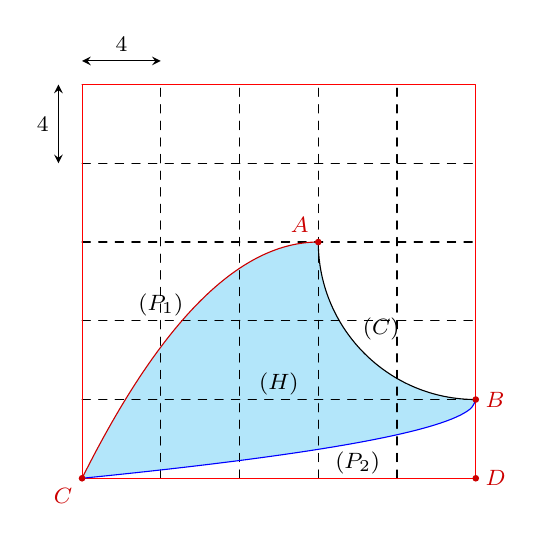
\begin{tikzpicture}[>=stealth,scale=1,line cap=round,line join=round,font=\footnotesize]
			\fill[cyan!30] (0,0) plot[domain=0:3,samples=100] (\x,{-1/3*(\x-3)^2+3}) arc (180:270:2) -- plot[domain=5:0,samples=100] (\x,{1-sqrt (1-\x/5)}) -- cycle;
			\draw[dashed] (0,0) grid (5,5);
			\draw[red] (0,0) rectangle (5,5);
			\draw[red!80!black,smooth] plot[domain=0:3,samples=100] (\x,{-1/3*(\x-3)^2+3});
			\draw[blue,smooth] plot[domain=0:5,samples=100] (\x,{1-sqrt (1-\x/5)});
			\draw (3,3) arc (180:270:2);
			\foreach \x/\y/\name in {1/2.2/P_1,3.5/0.2/P_2,3.8/1.9/C,2.5/1.2/H}
			\node at (\x,\y) {$(\name)$};
			\foreach \x/\y/\pos/\lbl in {0/0/below left/C,3/3/above left/A,5/1/right/B,5/0/right/D}
			\fill[red!80!black] (\x,\y) circle (1.2pt) node[\pos] {$\lbl$};
			\draw[<->] (0,5.3) -- (1,5.3) node[midway,above] {$4$};
			\draw[<->] (-0.3,4) -- (-0.3,5) node[midway,left] {$4$};
		\end{tikzpicture}
	}
	\par
	\shortans[0]{115}
	\loigiai{
		Chọn hệ trục tọa độ $Oxy$ với gốc tọa độ $O$ trùng với điểm $C(0;0)$, trục hoành chứa đoạn $CD$, trục tung chứa mép trái của lưới.\\
		Dựa vào thông tin lưới ô vuông (mỗi ô có kích thước $4 \times 4$), ta xác định được tọa độ các điểm $C(0;0)$, $A(12;12)$, $B(20;4)$, $D(20;0)$.\\
		\textbf{Cách 1: Phương pháp tọa độ (tích phân trực tiếp)}\\
		\textbf{1. Tìm phương trình các đường biên:}
		\begin{itemize}
			\item Đường parabol $(P_1)$: có đỉnh $A(12;12)$, trục đối xứng thẳng đứng nên có dạng \[y = a(x-12)^2 + 12.\] Vì $(P_1)$ đi qua gốc $C(0;0)$ nên ta có
			\[0 = a(0-12)^2 + 12 \Leftrightarrow 144a = -12 \Leftrightarrow a = -\dfrac{1}{12}. \]
			Suy ra $(P_1) \colon y = f(x) = -\dfrac{1}{12}(x-12)^2 + 12$ với $x \in [0;12]$.
			\item Đường parabol $(P_2)$: có đỉnh $B(20;4)$, trục đối xứng nằm ngang nên có dạng $x = a(y-4)^2 + 20$. Vì $(P_2)$ đi qua $C(0;0)$ nên ta có
			\[0 = a(0-4)^2 + 20 \Leftrightarrow 16a = -20 \Leftrightarrow a = -\dfrac{5}{4}. \]
			Suy ra $x = -\dfrac{5}{4}(y-4)^2 + 20 \Rightarrow (y-4)^2 = 16 - \dfrac{4}{5}x$.\\ Vì ta lấy nhánh dưới $y \in [0;4]$ nên $y-4 \le 0$, phương trình là
			\[(P_2) \colon y = g(x) = 4 - \sqrt{16 - \dfrac{4}{5}x} \quad \text{ với } x \in [0;20]. \]
			\item Cung tròn $(C)$: đi qua $A(12;12)$ và $B(20;4)$.\\ Tâm của cung tròn là $E(20;12)$ (đỉnh trên cùng bên phải lưới $5\times 3$), bán kính $R = EA = 8$.\\ Vì cung $(C)$ nằm phía dưới $E$ nên phương trình là
			\[y = h(x) = 12 - \sqrt{64 - (x-20)^2} \quad \text{ với } x \in [12;20]. \]
		\end{itemize}
		\textbf{2. Tính diện tích hình $(H)$:} \\
		Diện tích hình $(H)$ bằng phần diện tích nằm dưới các biên trên $(P_1)$, $(C)$ trừ đi phần diện tích dưới biên dưới $(P_2)$.\\ Ta có $S_{(H)} = S_{\text{ trên}} - S_{\text{ dưới}}$.
		\begin{itemize}
			\item
			\begin{align*}
				S_{\text{ trên}} &= \displaystyle\int\limits_{0}^{12} f(x) \mathrm{d}x + \int\limits_{12}^{20} h(x) \mathrm{d}x \\
				&= \int\limits_{0}^{12} \left[-\dfrac{1}{12}(x-12)^2 + 12 \right] \mathrm{d}x + \int\limits_{12}^{20} \left[12 - \sqrt{64 - (x-20)^2} \right] \mathrm{d}x\\
				&= \left(-\dfrac{1}{36}(x-12)^3 + 12x \right) \Bigg|_0^{12} + \left(96 - \dfrac{1}{4} \cdot \pi \cdot 8^2 \right) \\
				&= 96 + 96 - 16\pi \\
				&= 192 - 16\pi.
			\end{align*}
			\item $S_{\text{ dưới}} = \displaystyle\int\limits_{0}^{20} \left(4 - \sqrt{16 - \dfrac{4}{5}x} \right) \mathrm{d}x$.\\ Áp dụng công thức hàm hợp $\displaystyle\int (ax+b)^n \mathrm{d}x = \dfrac{1}{a} \cdot \dfrac{(ax+b)^{n+1}}{n+1}$, ta có
			\begin{align*}
				S_{\text{ dưới}} &= \left[4x - \dfrac{1}{-\frac{4}{5}} \cdot \dfrac{\left(16 - \frac{4}{5}x\right)^{\frac{3}{2}}}{\frac{3}{2}} \right] \Bigg|_0^{20} \\
				&= \left[4x + \dfrac{5}{6} \left(16 - \dfrac{4}{5}x\right)\sqrt{16 - \dfrac{4}{5}x} \right] \Bigg|_0^{20} \\
				&= (80 + 0) - \left(0 + \dfrac{5}{6} \cdot 16 \cdot \sqrt{16} \right) \\
				&= 80 - \dfrac{5}{6} \cdot 64 \\
				&= 80 - \dfrac{160}{3} = \dfrac{80}{3}.
			\end{align*}
		\end{itemize}
		Vậy $S_{(H)} = (192 - 16\pi) - \dfrac{80}{3} = \dfrac{496}{3} - 16\pi \approx 115{,}067 \approx 115$.\\
		\textbf{Cách 2: Phương pháp hình học (dùng công thức diện tích nhanh)}
		\immini{
			Dựng hình chữ nhật $CDEF$ ngoại tiếp toàn bộ hình phẳng $(H)$ với $E(20;12)$ và $F(0;12)$.\\ Hình chữ nhật này có chiều dài $20$ và chiều rộng $12$.\\
			Diện tích cần tìm được xác định bởi $S_{(H)} = S_{CDEF} - S_1 - S_2 - S_3$.\\
			Ta có $S_{CDEF} = 20 \cdot 12 = 240$.\\
			Sử dụng tính chất \textbf{\lq\lq Diện tích phần hình phẳng nằm ngoài parabol (từ đỉnh đến điểm giới hạn) bằng $\dfrac{1}{3}$ diện tích hình chữ nhật chứa nó\rq\rq}.
		}{
			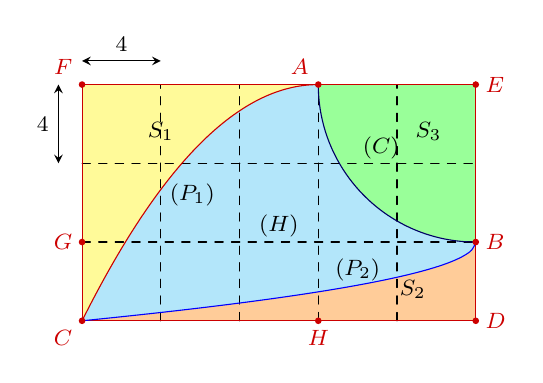
\begin{tikzpicture}[>=stealth,scale=1,line cap=round,line join=round,font=\footnotesize]
				\fill[cyan!30] (0,0) plot[domain=0:3,samples=100] (\x,{-1/3*(\x-3)^2+3}) arc (180:270:2) -- plot[domain=5:0,samples=100] (\x,{1-sqrt (1-\x/5)}) -- cycle;
				\fill[yellow!40] (0,0) plot[domain=0:3,samples=100] (\x,{-1/3*(\x-3)^2+3}) -- (0,3) -- cycle;
				\fill[orange!40] (0,0) plot[domain=0:5,samples=100] (\x,{1-sqrt (1-\x/5)}) -- (5,0) -- cycle;
				\fill[green!40] (3,3) arc (180:270:2) -- (5,3) -- cycle;
				\draw[dashed] (0,0) grid (5,3);
				\draw[red!80!black] (0,0) rectangle (5,3);
				\draw[red!80!black] plot[domain=0:3,samples=100] (\x,{-1/3*(\x-3)^2+3});
				\draw[blue,smooth] plot[domain=0:5,samples=100] (\x,{1-sqrt (1-\x/5)});
				\draw[blue!40!black] (3,3) arc (180:270:2);
				\foreach \x/\y/\name in {1.4/1.6/P_1,3.5/0.65/P_2,3.8/2.2/C,2.5/1.2/H}
				\node at (\x,\y) {$(\name)$};
				\foreach \x/\y/\name in {1/2.4/S_1,4.2/0.4/S_2,4.4/2.4/S_3}
				\node at (\x,\y) {$\name$};
				\foreach \x/\y/\pos/\lbl in {0/0/below left/C,3/3/above left/A,5/1/right/B,5/0/right/D,5/3/right/E,0/3/above left/F,0/1/left/G,3/0/below/H}
				\fill[red!80!black] (\x,\y) circle (1.2pt) node[\pos] {$\lbl$};
				\draw[<->] (0,3.3) -- (1,3.3) node[midway,above] {$4$};
				\draw[<->] (-0.3,2) -- (-0.3,3) node[midway,left] {$4$};
			\end{tikzpicture}
		}
		$S_1$ là phần nằm ngoài của parabol $(P_1)$ trong hình chữ nhật $CHAF$ có kích thước $12 \times 12$. Do đó
		\[S_1 = \dfrac{1}{3} S_{CHAF} = \dfrac{1}{3} \cdot 12 \cdot 12 = 48.\]
		$S_2$ là phần nằm ngoài của parabol $(P_2)$ trong hình chữ nhật $CDBG$ có kích thước $20 \times 4$. Do đó
		\[S_2 = \dfrac{1}{3} S_{CDBG} = \dfrac{1}{3} \cdot 20 \cdot 4 = \dfrac{80}{3}.\]
		$S_3$ là diện tích một phần tư hình tròn tâm $E(20;12)$, bán kính $R = EA = 8$. Do đó
		\[S_3 = \dfrac{1}{4} \pi R^2 = \dfrac{1}{4} \pi \cdot 8^2 = 16\pi.\]
		Vậy diện tích hình phẳng $(H)$ là
		\[S_{(H)} = 240 - 48 - \dfrac{80}{3} - 16\pi = \dfrac{496}{3} - 16\pi \approx 115. \]
	}
\end{ex}
%%%=============================%%%

%%%=============EX_19=============%%%
\begin{ex}%[1H8V6-2]%[TDMT15]%[Duong Xuan Loi]
	Cho hình chóp $S.ABC$ có $\widehat{ASB}=60^\circ$, $\widehat{BSC}=50^\circ$, $\widehat{CSA}=40^\circ$. Hãy xác định số đo của góc nhị diện $[A,SB,C]$ theo đơn vị độ (\textit{làm tròn đến hàng đơn vị}).
	\par
	\shortans[0]{48}
	\loigiai{
		\begin{center}
			\begin{tikzpicture}[declare function={
					xC=-3.5; yC=0.5;
					xB=3.5; yB=1.5;
					xS=1.5; yS=-1.5;
					xH=-0.5; yH=0.4;
					h=4.5;
					tN=0.65; tM=0.35;
					shiftX=8.5; shiftY=-1.5;
					angM=65; angN=115; distH=2.5; rayL=3.5;
				},line join=round,line cap=round,ethicknode/.style={font=\large}]
				\path
				(xC,yC) coordinate (C)
				(xB,yB) coordinate (B)
				(xS,yS) coordinate (S)
				(xH,yH) coordinate (H);
				\path ($(H)+(0,h)$) coordinate (A);
				\path ($(C)!tN!(S)$) coordinate (N);
				\path ($(S)!tM!(B)$) coordinate (M);
				\draw[line width=0.6pt] (A) -- (C)
				(A) -- (S)
				(A) -- (B)
				(C) -- (S) -- (B)
				(A) -- (N)
				(A) -- (M);
				\draw[dashed,line width=0.6pt] (C) -- (B)
				(A) -- (H)
				(H) -- (N)
				(H) -- (M);
				\path pic[draw,dashed,line width=0.6pt,angle radius=12pt] {angle=B--S--C};
				\foreach \p/\pos in {C/225,B/0,S/-90,H/-135,A/90,N/-90,M/0}{
					\draw (\p) circle (0.6pt) node[shift={(\pos:8pt)}] {$\p$};
				}
				\path
				(shiftX,shiftY) coordinate (S2)
				(S2) ++(angN:rayL) coordinate (RayN)
				(S2) ++(angM:rayL) coordinate (RayM)
				(S2) ++({(angN+angM)/2}:distH) coordinate (H2)
				($(S2)!(H2)!(RayN)$) coordinate (N2)
				($(S2)!(H2)!(RayM)$) coordinate (M2);
				\draw[line width=0.6pt] (S2) -- (RayN)
				(S2) -- (RayM)
				(S2) -- (H2)
				(H2) -- (N2)
				(H2) -- (M2);
				\path pic[draw,dashed,line width=0.6pt,angle radius=15pt] {angle=RayM--S2--RayN};
				\node[right] at ($(S2)+(30:15pt)$) {$50^\circ$};
				\foreach \p/\pos/\label in {S2/-90/S,N2/180/N,H2/90/H,M2/0/M}{
					\draw (\p) circle (0.6pt) node[shift={(\pos:8pt)}] {$\label$};
				}
			\end{tikzpicture}
		\end{center}
		\textbf{Bước 1: Xác định góc nhị diện}\\
		Gọi $H$ là hình chiếu vuông góc của $A$ lên mặt phẳng $(SBC)$.\\
		Kẻ $AM \perp SB$ tại $M$ và $AN \perp SC$ tại $N$.
		Ta có
		\[\heva{& SB \perp AH \text{ (do } AH \perp (SBC)) \\ & SB \perp AM} \Rightarrow SB \perp (AHM) \Rightarrow SB \perp HM. \]
		Do $AM \perp SB$ và $HM \perp SB$, nên số đo góc nhị diện $[A,SB,C]$ chính là số đo của góc $\widehat{AMH}$.\\
		Tương tự, ta cũng chứng minh được $SC \perp (AHN) \Rightarrow SC \perp HN$.\\
		\textbf{Bước 2: Tính các đại lượng liên quan}\\
		Trong mặt phẳng $(SBC)$, xét tứ giác $SMHN$ có $\widehat{SMH} = \widehat{SNH} = 90^\circ$ nên $SMHN$ là tứ giác nội tiếp đường tròn đường kính $SH$.\\
		Áp dụng định lí sin cho $\triangle SMN$ nội tiếp đường tròn đường kính $SH$, ta có
		\[\dfrac{MN}{\sin \widehat{MSN}} = SH \Rightarrow SH = \dfrac{MN}{\sin 50^\circ}. \]
		Xét các tam giác vuông $SAM$ và $SAN$, ta có
		\[\heva{& AM = SA \cdot \sin \widehat{ASB} = SA \cdot \sin 60^\circ \\ & SM = SA \cdot \cos \widehat{ASB} = SA \cdot \cos 60^\circ\\& AN = SA \cdot \sin \widehat{CSA} = SA \cdot \sin 40^\circ \\ & SN = SA \cdot \cos \widehat{CSA} = SA \cdot \cos 40^\circ.} \]
		Áp dụng định lí côsin cho $\triangle SMN$ ta có
		\begin{align*}
			MN &= \sqrt{SM^2 + SN^2 - 2 \cdot SM \cdot SN \cdot \cos \widehat{MSN}} \\
			&= \sqrt{(SA\cos 60^\circ)^2 + (SA\cos 40^\circ)^2 - 2(SA\cos 60^\circ)(SA\cos 40^\circ)\cos 50^\circ} \\
			&= SA \sqrt{\cos^2 60^\circ + \cos^2 40^\circ - 2\cos 60^\circ \cos 40^\circ \cos 50^\circ}.
		\end{align*}
		Suy ra
		\[SH = \dfrac{SA \sqrt{\cos^2 60^\circ + \cos^2 40^\circ - 2\cos 60^\circ \cos 40^\circ \cos 50^\circ}}{\sin 50^\circ}. \]
		Xét $\triangle SAH$ vuông tại $H$, áp dụng định lí Pythagore ta có
		\begin{align*}
			AH &= \sqrt{SA^2 - SH^2} \\
			&= \sqrt{SA^2 - SA^2 \dfrac{\cos^2 60^\circ + \cos^2 40^\circ - 2\cos 60^\circ \cos 40^\circ \cos 50^\circ}{\sin^2 50^\circ}} \\
			&= SA \sqrt{\dfrac{\sin^2 50^\circ - \cos^2 60^\circ - \cos^2 40^\circ + 2\cos 60^\circ \cos 40^\circ \cos 50^\circ}{\sin^2 50^\circ}}.
		\end{align*}
		\textbf{Bước 3: Tính góc nhị diện}\\
		Xét tam giác vuông $AHM$ (vuông tại $H$), ta có $\sin \widehat{AMH} = \dfrac{AH}{AM}$.\\ Thay các kết quả vừa tính được vào, ta được
		\begin{align*}
			\sin \widehat{AMH} &= \dfrac{SA \dfrac{\sqrt{\sin^2 50^\circ - \cos^2 60^\circ - \cos^2 40^\circ + 2\cos 60^\circ \cos 40^\circ \cos 50^\circ}}{\sin 50^\circ}}{SA \cdot \sin 60^\circ} \\
			&= \dfrac{\sqrt{\sin^2 50^\circ - \cos^2 60^\circ - \cos^2 40^\circ + 2\cos 60^\circ \cos 40^\circ \cos 50^\circ}}{\sin 50^\circ \cdot \sin 60^\circ}\\
			\Rightarrow \widehat{AMH} &\approx 48^\circ.
		\end{align*}
		Vậy số đo của góc nhị diện $[A,SB,C]$ là $48^\circ$.
	}
\end{ex}
%%%=============================%%%

%%%=============EX_20=============%%%
\begin{ex}%[1H3V2-2]%[TDMT15]%[Lê Hồ Quang Minh]
	Một hồ nước có bờ hồ là đường thẳng. Ở giữa có hai mảnh đất $A$ và $B$ được coi như hai hình tròn có cùng bán kính bằng $10$\,m, có hai tâm lần lượt là $A$ và $B$, khoảng cách từ hai tâm $A$ và $B$ đến bờ hồ lần lượt là $14$ m và $25$ m, khoảng cách giữa hai tâm là $32$ m. Người ta muốn mắc một đường dây từ một điểm $M$ thuộc rìa mô đất $A$ đến một điểm $P$ của bờ hồ rồi từ điểm $P$ của bờ hồ đến một điểm $N$ thuộc rìa mô đất $B$. Gọi $H$ và $K$ lần lượt là hai điểm trên bờ hồ gần với hai tâm của $A$ và $B$ nhất, điểm $P$ nằm trong đoạn $HK$. Hãy tính giá trị ngắn nhất của đường dây theo đơn vị mét \textit{(làm tròn kết quả đến hàng phần chục)}.
	\par
	\shortans[0]{29,2}
	\loigiai{
		\begin{center}
			\begin{tikzpicture}[>=stealth,line join=round,line cap=round,font=\footnotesize,scale=0.2]
				\coordinate (K) at (0,0);
				\coordinate (H) at (30.05,0);
				\coordinate (B) at (0,25);
				\coordinate (A) at (30.05,14);
				\coordinate (P) at (19.26,0);
				\coordinate (L) at (0,14);
				\fill[cyan!50,opacity=.8] (B) circle (10);
				\fill[cyan!50,opacity=.8] (A) circle (10);
				\draw[red!60!black] (-5,0) -- (35,0);
				\draw[dashed] (B) -- (K) node[midway,left] {$25$};
				\draw[dashed] (A) -- (H) node[midway,right] {$14$};
				\draw[dashed] (B) -- (A) node[midway,above] {$32$};
				\draw[dashed] (L) -- (A);
				\draw (B) circle (10);
				\draw (A) circle (10);
				\coordinate (N) at ($(B)!0.317!(P)$);
				\coordinate (M) at ($(A)!0.566!(P)$);
				\coordinate (M') at ($(A)+(245:10)$);
				\draw[red!60!black] (M) -- (P) -- (N);
				\draw[red!60!black] (P) -- (M');
				\draw[thin] (B) -- (N);
				\draw[thin] (A) -- (M);
				\draw[thin] (M') -- (A);
				\fill (K) circle (5 pt) node[below=3 pt] {$K$};
				\fill (H) circle (5 pt) node[below=3 pt] {$H$};
				\fill (P) circle (5 pt) node[below=3 pt] {$P$};
				\fill (B) circle (5 pt) node[left=3 pt] {$B$};
				\fill (A) circle (5 pt) node[right=3 pt] {$A$};
				\fill (N) circle (5 pt) node[right] {$N$};
				\fill (M) circle (5 pt) node[left] {$M$};
				\fill (M') circle (5 pt) node[below] {$M'$};
				\fill (L) circle (5 pt) node[below right] {$L$};
				\path (P) -- (H) node[midway,below] {$x$};
			\end{tikzpicture}
		\end{center}
		Gọi $d$ là đường thẳng bờ hồ.\\ Vì $H$, $K$ là hai điểm trên bờ hồ gần với hai tâm $A$, $B$ nhất nên $H$, $K$ lần lượt là hình chiếu vuông góc của $A$, $B$ lên $d$. \\
		Ta có $AH = 14$, $BK = 25$, $AB = 32$.\\ Kẻ $AL \perp BK$ tại $L$, ta có hình chữ nhật $ALKH$, suy ra
		\[HK = \sqrt{AB^2 - (BK - AH)^2} = \sqrt{32^2 - (25-14)^2} = \sqrt{903}. \]
		Độ dài đường dây cần thiết lập là $S = PM + PN$. \\
		Với mọi vị trí của $M$ trên đường tròn $(A)$ và $N$ trên đường tròn $(B)$, ta luôn có
		\[\heva{&PM \ge PA - R_A = PA - 10 \\& PN \ge PB - R_B = PB - 10.} \]
		Suy ra $S = PM + PN \ge PA + PB - 20$.\\ Dấu đẳng thức xảy ra khi $A$, $M$, $P$ thẳng hàng và $B$, $N$, $P$ thẳng hàng.\\
		Đặt $x = PH$ với $x \in \left(0; \sqrt{903}\right)$, suy ra $PK = \sqrt{903} - x$. \\
		Khi đó $PA = \sqrt{PH^2 + AH^2} = \sqrt{x^2 + 196}$ và $PB = \sqrt{PK^2 + BK^2} = \sqrt{\left(\sqrt{903}-x\right)^2 + 625}$. \\
		Bài toán quy về tìm giá trị nhỏ nhất của hàm số
		\[f(x) = \sqrt{x^2 + 196} + \sqrt{\left(\sqrt{903}-x\right)^2 + 625} - 20 \quad \text{ trên khoảng } \left(0; \sqrt{903}\right). \]
		Ta có
		\[f'(x) = \dfrac{x}{\sqrt{x^2 + 196}} - \dfrac{\sqrt{903}-x}{\sqrt{\left(\sqrt{903}-x\right)^2 + 625}}. \]
		Xét phương trình $f'(x) = 0 \Leftrightarrow \dfrac{x}{\sqrt{x^2 + 196}} = \dfrac{\sqrt{903}-x}{\sqrt{\left(\sqrt{903}-x\right)^2 + 625}}$.\\
		Bình phương hai vế và nhân chéo (do $x > 0$ và $\sqrt{903}-x > 0$), ta được
		\begin{align*}
			x^2\left[\left(\sqrt{903}-x\right)^2 + 625 \right] &= \left(\sqrt{903}-x\right)^2 (x^2 + 196) \\
			625 x^2 &= 196\left(\sqrt{903}-x\right)^2 \\
			25 x &= 14(\sqrt{903}-x) \\
			39 x &= 14\sqrt{903} \\
			x &= \dfrac{14\sqrt{903}}{39} \approx 10{,}787 \in \left(0; \sqrt{903}\right).
		\end{align*}
		Đặt $x_0 = \dfrac{14\sqrt{903}}{39}$.\\ Ta có bảng biến thiên của hàm số $f(x)$
		\begin{center}
			
\begin{tikzpicture}
				\tkzTabInit[nocadre=false,lgt=1.5,espcl=4]{$x$ / 1,$f'(x)$ / 1,$f (x)$ / 2.5}{$0$,$x_0$,$\sqrt{903}$}
				\tkzTabLine{,-,0,+,}
				\tkzTabVar{+/,-/ $f (x_0)$,+/}
			\end{tikzpicture}
		\end{center}
		Dựa vào bảng biến thiên, hàm số đạt giá trị nhỏ nhất tại $x = x_0$. \\
		Thay $x_0$ vào $f(x)$, ta được
		\[\min f(x) = f(x_0) = \sqrt{2\,424} - 20 \approx 29{,}2. \]
		Vậy giá trị ngắn nhất của đường dây xấp xỉ $29{,}2$ m.
	}
\end{ex}
%%%=============================%%%

%%%=============EX_21=============%%%
\begin{ex}%[2H5V2-7]%[TDMT15]%[Nguyễn Văn Sang]
	\immini[thm]
	{Gắn hệ trục toạ độ $Oxyz$ với mặt đất là mặt phẳng toạ độ $(Oxy)$ và đơn vị độ dài trên mỗi trục là $1$\,km, trục $Ox$ hướng về nam, trục $Oy$ hướng về đông. Tại một thời điểm người ta quan sát thấy có hai khinh khí cầu X và Y lần lượt có toạ độ $X(4;3;2)$ và $Y(-2;-1;7)$. Quan sát và nhận ra khinh khí cầu X đang bay về phía tây với tốc độ không đổi bằng $30$\,km/h, khinh khí cầu Y đang bay về phía nam với tốc độ không đổi $40$\,km/h, đồng thời cả hai khinh khí cầu đều chếch xuống so với phương ngang một góc $\varphi$ $\left(\tan\varphi=0{,}1\right)$. Hãy tính khoảng cách nhỏ nhất giữa hai khinh khí cầu đơn vị kilômet (\textit{làm tròn kết quả đến hàng phần trăm}).}
	{\begin{tikzpicture}[x={(-0.6 cm,-0.4 cm)},y={(1 cm,0 cm)},z={(0 cm,1 cm)},scale=0.8,font=\footnotesize,line join=round,line cap=round]
			\draw[->,black!80] (0,0,0) -- (6,0,0) node[below left] {$x$(Nam)};
			\draw[->,black!80] (0,0,0) -- (0,5,0) node[right] {$y$(Đông)};
			\draw[->,black!80] (0,0,0) -- (0,0,8.5) node[above] {$z$(Trời)};
			\node[below right] at (0,0,0) {$O$};
			\draw[dashed,gray!80] (0,0,0) -- (-3,0,0);
			\draw[dashed,gray!80] (0,0,0) -- (0,-2,0);
			\coordinate (X) at (4,3,2);
			\draw[dashed,teal!80] (4,0,0) -- (4,3,0) -- (0,3,0);
			\draw[dashed,teal!80] (0,0,2) -- (4,0,2) -- (X) -- (0,3,2) -- cycle;
			\draw[dashed,teal!80] (4,0,0) -- (4,0,2);
			\draw[dashed,teal!80] (4,3,0) -- (X);
			\draw[dashed,teal!80] (0,3,0) -- (0,3,2);
			\fill[teal] (X) circle (3 pt) node[right=4 pt] {$X (4; 3; 2)$};
			\draw[->,blue!80!black] (X) -- ++(0,-2.5,-0.5) node[midway,above] {$\overrightarrow{v}_X$};
			\coordinate (Y) at (-2,-1,7);
			\draw[dashed,orange!80] (-2,0,0) -- (-2,-1,0) -- (0,-1,0);
			\draw[dashed,orange!80] (0,0,7) -- (-2,0,7) -- (Y) -- (0,-1,7) -- cycle;
			\draw[dashed,orange!80] (-2,0,0) -- (-2,0,7);
			\draw[dashed,orange!80] (-2,-1,0) -- (Y);
			\draw[dashed,orange!80] (0,-1,0) -- (0,-1,7);
			\fill[orange!80!black] (Y) circle (3 pt) node[left=4 pt] {$Y (-2; -1; 7)$};
			\draw[->,blue!80!black] (Y) -- ++(2.5,0,-0.5) node[midway,left] {$\overrightarrow{v}_Y$};
		\end{tikzpicture}
	}
	\par
	\shortans[0]{4,87}
	\loigiai{
		Gọi $t$ ($t \ge 0$) là thời gian (giờ) tính từ lúc quan sát ban đầu.\\
		Theo hệ trục tọa độ đã chọn, hướng nam là chiều dương của trục $Ox$, hướng đông là chiều dương của trục $Oy$, hướng lên trời là chiều dương của trục $Oz$.\\
		Vectơ đơn vị theo hướng nam là $\overrightarrow{i} = (1; 0; 0)$ và theo hướng tây là $-\overrightarrow{j} = (0; -1; 0)$.\\
		Khinh khí cầu X di chuyển về phía tây và chếch xuống dưới một góc $\varphi$ với $\tan\varphi = 0{,}1$, do đó vectơ chỉ hướng của X là $\overrightarrow{u} = -\overrightarrow{j} - 0{,}1\overrightarrow{k} = (0; -1; -0{,}1)$.\\
		Độ dài của vectơ $\overrightarrow{u}$ là $\left|\overrightarrow{u}\right| = \sqrt{0^2 + (-1)^2 + (-0{,}1)^2} = \dfrac{\sqrt{101}}{10}$.\\
		Vì X di chuyển với tốc độ $30$ km/h nên quãng đường đi được sau thời gian $t$ là $30 t$.\\ Gọi $M$ là vị trí của X ở thời điểm $t$, ta có sự dịch chuyển của X được xác định bởi
		\[\overrightarrow{XM} = \dfrac{30 t}{\left|\overrightarrow{u}\right|}\overrightarrow{u} = \dfrac{300 t}{\sqrt{101}}(0; -1; -0{,}1) \Rightarrow M\left(4; 3 - \dfrac{300 t}{\sqrt{101}}; 2 - \dfrac{30 t}{\sqrt{101}}\right). \]
		Khinh khí cầu Y di chuyển về phía nam và chếch xuống dưới một góc $\varphi$, do đó vectơ chỉ hướng của Y là $\overrightarrow{v} = \overrightarrow{i} - 0{,}1\overrightarrow{k} = (1; 0; -0{,}1)$.\\
		Tương tự, độ dài của vectơ $\overrightarrow{v}$ là $|\overrightarrow{v}| = \dfrac{\sqrt{101}}{10}$.\\
		Vì Y di chuyển với tốc độ $40$ km/h nên quãng đường đi được sau thời gian $t$ là $40 t$. Gọi $N$ là vị trí của Y ở thời điểm $t$, ta có sự dịch chuyển của Y được xác định bởi
		\[\overrightarrow{YN} = \dfrac{40 t}{\left|\overrightarrow{v}\right|}\overrightarrow{v} = \dfrac{400 t}{\sqrt{101}}(1; 0; -0{,}1) \Rightarrow N\left(-2 + \dfrac{400 t}{\sqrt{101}}; -1; 7 - \dfrac{40 t}{\sqrt{101}}\right). \]
		Bình phương khoảng cách giữa hai khinh khí cầu tại thời điểm $t$ là
		\[MN^2 = \left(\dfrac{400 t}{\sqrt{101}} - 6 \right)^2 + \left(\dfrac{300 t}{\sqrt{101}} - 4 \right)^2 + \left(\dfrac{10 t}{\sqrt{101}} - 5 \right)^2. \]
		Khai triển và rút gọn biểu thức trên, ta được hàm số theo biến $t$
		\[f(t) = \dfrac{250\,100}{101}t^2 - \dfrac{7\,300}{\sqrt{101}}t + 77. \]	
		Hàm số $f(t)$ là một parabol có bề lõm hướng lên trên (do hệ số $a > 0$), nên đạt giá trị nhỏ nhất tại hoành độ đỉnh $t = -\dfrac{b}{2 a} = \dfrac{73\sqrt{101}}{5\,002}$.\\
		Thay giá trị $t$ này vào hàm số, ta tìm được khoảng cách bình phương nhỏ nhất là
		\[\min f(t) = f\left(\dfrac{73\sqrt{101}}{5\,002} \right) = \dfrac{59\,352}{2\,501}. \]
		Vậy khoảng cách nhỏ nhất giữa hai khinh khí cầu là $MN_{\min} = \sqrt{\dfrac{59\,352}{2\,501}} \approx 4{,}87$ (km).
	}
\end{ex}
%%%=============================%%%

%%%=============EX_22=============%%%
\begin{ex}%[1D2V3-2]%[TDMT15]%[Nguyễn Thành Hậu]
	Bỏ ngẫu nhiên $7$ viên bi có cùng kích thước và khối lượng vào $4$ chiếc hộp khác nhau, trong đó có hai viên bi màu đỏ được đánh số $1$ và $2$, hai viên bi màu xanh được đánh số $1$ và $2$, một viên bi màu vàng, một viên bi màu tím, một viên bi màu đen. Gọi $p$ là xác suất để không có hai viên bi cùng màu nào ở chung một hộp và mỗi hộp có ít nhất một viên bi. Hãy tính $1\,000p$ (\textit{làm tròn kết quả đến hàng đơn vị}).
	\begin{center}
		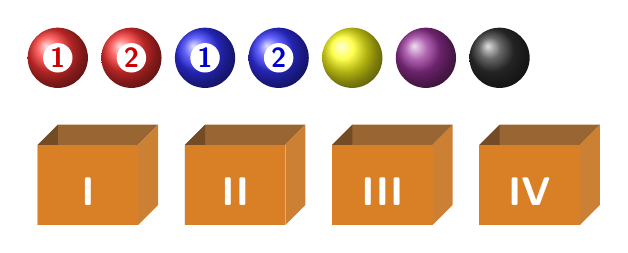
\begin{tikzpicture}[scale=0.85,font=\sffamily]
			% Lệnh vẽ hộp 3D đơn giản
			\def\drawbox#1#2{
				\begin{scope}[shift={(#1,0)}]
					% Mặt trong (phía sau và đáy)
					\fill[brown!80!black] (0,1.2) -- (0.3,1.5) -- (1.8,1.5) -- (1.5,1.2) -- cycle;
					\fill[brown!60!black] (0,0) -- (0.3,0.3) -- (0.3,1.5) -- (0,1.2) -- cycle;
					% Mặt ngoài (phải và trước)
					\fill[brown!80!orange] (1.5,0) -- (1.8,0.3) -- (1.8,1.5) -- (1.5,1.2) -- cycle;
					\fill[brown!60!orange] (0,0) rectangle (1.5,1.2);
					% Nhãn hộp
					\node[white] at (0.75,0.5) {\Large\textbf{#2}};
				\end{scope}
			}
			% Vẽ 4 hộp
			\drawbox{0}{I}
			\drawbox{2.2}{II}
			\drawbox{4.4}{III}
			\drawbox{6.6}{IV}
			% Vẽ 7 viên bi
			% Bi Đỏ 1
			\begin{scope}[shift={(0.3,2.5)}]
				\shade[ball color=red!80!white] (0,0) circle (0.45);
				\fill[white] (0,0) circle (0.22);
				\node[red!80!black] at (0,0) {\textbf{1}};
			\end{scope}
			% Bi Đỏ 2
			\begin{scope}[shift={(1.4,2.5)}]
				\shade[ball color=red!80!white] (0,0) circle (0.45);
				\fill[white] (0,0) circle (0.22);
				\node[red!80!black] at (0,0) {\textbf{2}};
			\end{scope}
			% Bi Xanh 1
			\begin{scope}[shift={(2.5,2.5)}]
				\shade[ball color=blue!80!white] (0,0) circle (0.45);
				\fill[white] (0,0) circle (0.22);
				\node[blue!80!black] at (0,0) {\textbf{1}};
			\end{scope}
			% Bi Xanh 2
			\begin{scope}[shift={(3.6,2.5)}]
				\shade[ball color=blue!80!white] (0,0) circle (0.45);
				\fill[white] (0,0) circle (0.22);
				\node[blue!80!black] at (0,0) {\textbf{2}};
			\end{scope}
			% Bi Vàng
			\begin{scope}[shift={(4.7,2.5)}]
				\shade[ball color=yellow!90!white] (0,0) circle (0.45);
			\end{scope}
			% Bi Tím
			\begin{scope}[shift={(5.8,2.5)}]
				\shade[ball color=violet!80!white] (0,0) circle (0.45);
			\end{scope}
			% Bi Đen
			\begin{scope}[shift={(6.9,2.5)}]
				\shade[ball color=black!80!white] (0,0) circle (0.45);
			\end{scope}
		\end{tikzpicture}
	\end{center}
	\par
	\shortans[0]{337}
	\loigiai{
		Phép thử: Xếp ngẫu nhiên $7$ viên bi phân biệt vào $4$ hộp khác nhau.\\ Mỗi viên bi có $4$ cách chọn hộp.
		\\ Không gian mẫu có số phần tử là $n(\Omega) = 4^7 = 16\,384$.\\		
		Gọi biến cố $A$: \textit{\lq\lq Không có hai viên bi cùng màu nào ở chung một hộp và mỗi hộp có ít nhất một viên bi\rq\rq\ }.\\
		Trước hết, ta đếm số cách xếp thỏa mãn điều kiện \lq\lq không có hai viên bi cùng màu chung hộp\rq\rq\  (gọi là tập $X$):
		\begin{itemize}
			\item Xếp $2$ viên bi đỏ vào $4$ hộp (sao cho mỗi hộp tối đa $1$ viên) có $\mathrm{A}_4^2 = 12$ cách.
			\item Xếp $2$ viên bi xanh vào $4$ hộp (sao cho mỗi hộp tối đa $1$ viên) có $\mathrm{A}_4^2 = 12$ cách.
			\item Xếp $3$ viên bi còn lại (vàng, tím, đen) vào $4$ hộp một cách tùy ý có $4 \cdot 4 \cdot 4 = 4^3$ cách.
		\end{itemize}
		Số cách xếp thỏa mãn điều kiện màu sắc là $n(X) = 12 \cdot 12 \cdot 64 = 9\,216$ cách.\\
		Tiếp theo, ta đi đếm phần bù, tức là đếm số cách xếp \textbf{vi phạm} điều kiện \lq\lq mỗi hộp có ít nhất một viên bi\rq\rq\  trong tập $X$. Vì có $2$ viên bi đỏ bắt buộc phải nằm ở $2$ hộp khác nhau, nên số hộp trống tối đa chỉ có thể là $2$.\\ Ta xét các trường hợp vi phạm:\\
		\textbf{Trường hợp 1:} Có đúng $2$ hộp bị bỏ trống.
		\begin{itemize}
			\item Chọn $2$ hộp để trống có $\mathrm{C}_4^2 = 6$ cách.
			\item Xếp $7$ viên bi vào $2$ hộp còn lại sao cho không có bi cùng màu chung hộp
			\begin{itemize}
				\item Xếp $2$ bi đỏ vào $2$ hộp: $\mathrm{A}_2^2$ cách.
				\item Xếp $2$ bi xanh vào $2$ hộp: $\mathrm{A}_2^2$ cách.
				\item Xếp $3$ bi (vàng, tím, đen) vào $2$ hộp: $2^3$ cách.
			\end{itemize}
			$\Rightarrow$ Số cách xếp bi là $\mathrm{A}_2^2 \cdot \mathrm{A}_2^2 \cdot 2^3 = 32$ cách.
		\end{itemize}
		Suy ra số cách vi phạm ở \textbf{Trường hợp $1$} là $6 \cdot 32 = 192$ cách.\\
		\textbf{Trường hợp 2:} Có đúng $1$ hộp bị bỏ trống.
		\begin{itemize}
			\item Chọn $1$ hộp để trống có $\mathrm{C}_4^1 = 4$ cách.
			\item Xếp $7$ viên bi vào $3$ hộp còn lại sao cho không có bi cùng màu chung hộp.\\ Số cách xếp tùy ý (có thể sinh ra hộp trống) là $\mathrm{A}_3^2 \cdot \mathrm{A}_3^2 \cdot 3^3 = 972$ cách.
			\item Tuy nhiên, trong $972$ cách này đã bao gồm cả các cách xếp mà \textbf{có thêm một hộp bị trống} (tức là bi chỉ được xếp vào $2$ trong $3$ hộp).\\ Số khả năng này chính là $\mathrm{C}_3^1 \cdot \left(\mathrm{A}_2^2 \cdot \mathrm{A}_2^2 \cdot 2^3\right) = 3 \cdot 32 = 96$ cách.
			\item Vậy số cách xếp để mỗi hộp trong $3$ hộp đều có bi là $972 - 96 = 876$ cách.
		\end{itemize}
		Suy ra số cách vi phạm ở \textbf{Trường hợp $2$} là $4 \cdot 876 = 3 504$ cách.\\
		Từ đó, số kết quả thuận lợi cho biến cố $A$ là
		\begin{align*}
			n(A) = 9\,216 - 192 - 3\,504 = 5\,520. 
		\end{align*}
		Xác suất của biến cố $A$ là
		\begin{align*}
			\mathrm{p} = \mathrm{P}(A) = \dfrac{n(A)}{n(\Omega)} = \dfrac{5\,520}{4^7} = \dfrac{345}{1\,024} \approx 0{,}3369. 
		\end{align*}
		Vậy $1\,000 p \approx 337$.
	}
\end{ex}
%%%=============================%%%
\Closesolutionfile{ans}

\newpage
\indapan{12}{ans/ansTN-Dung}
\indapan[TF]{2}{ans/ansTN-DungSai}
\indapan[SA]{6}{ans/ansTN-DienKhuyet}
%%%%%%%%%%%%%%
%%nhãn kết thúc đề (để đếm số trang tự động mỗi đề)
\label{B\thedeso}